% \begin{figure}[h!]
% \begin{center}
% 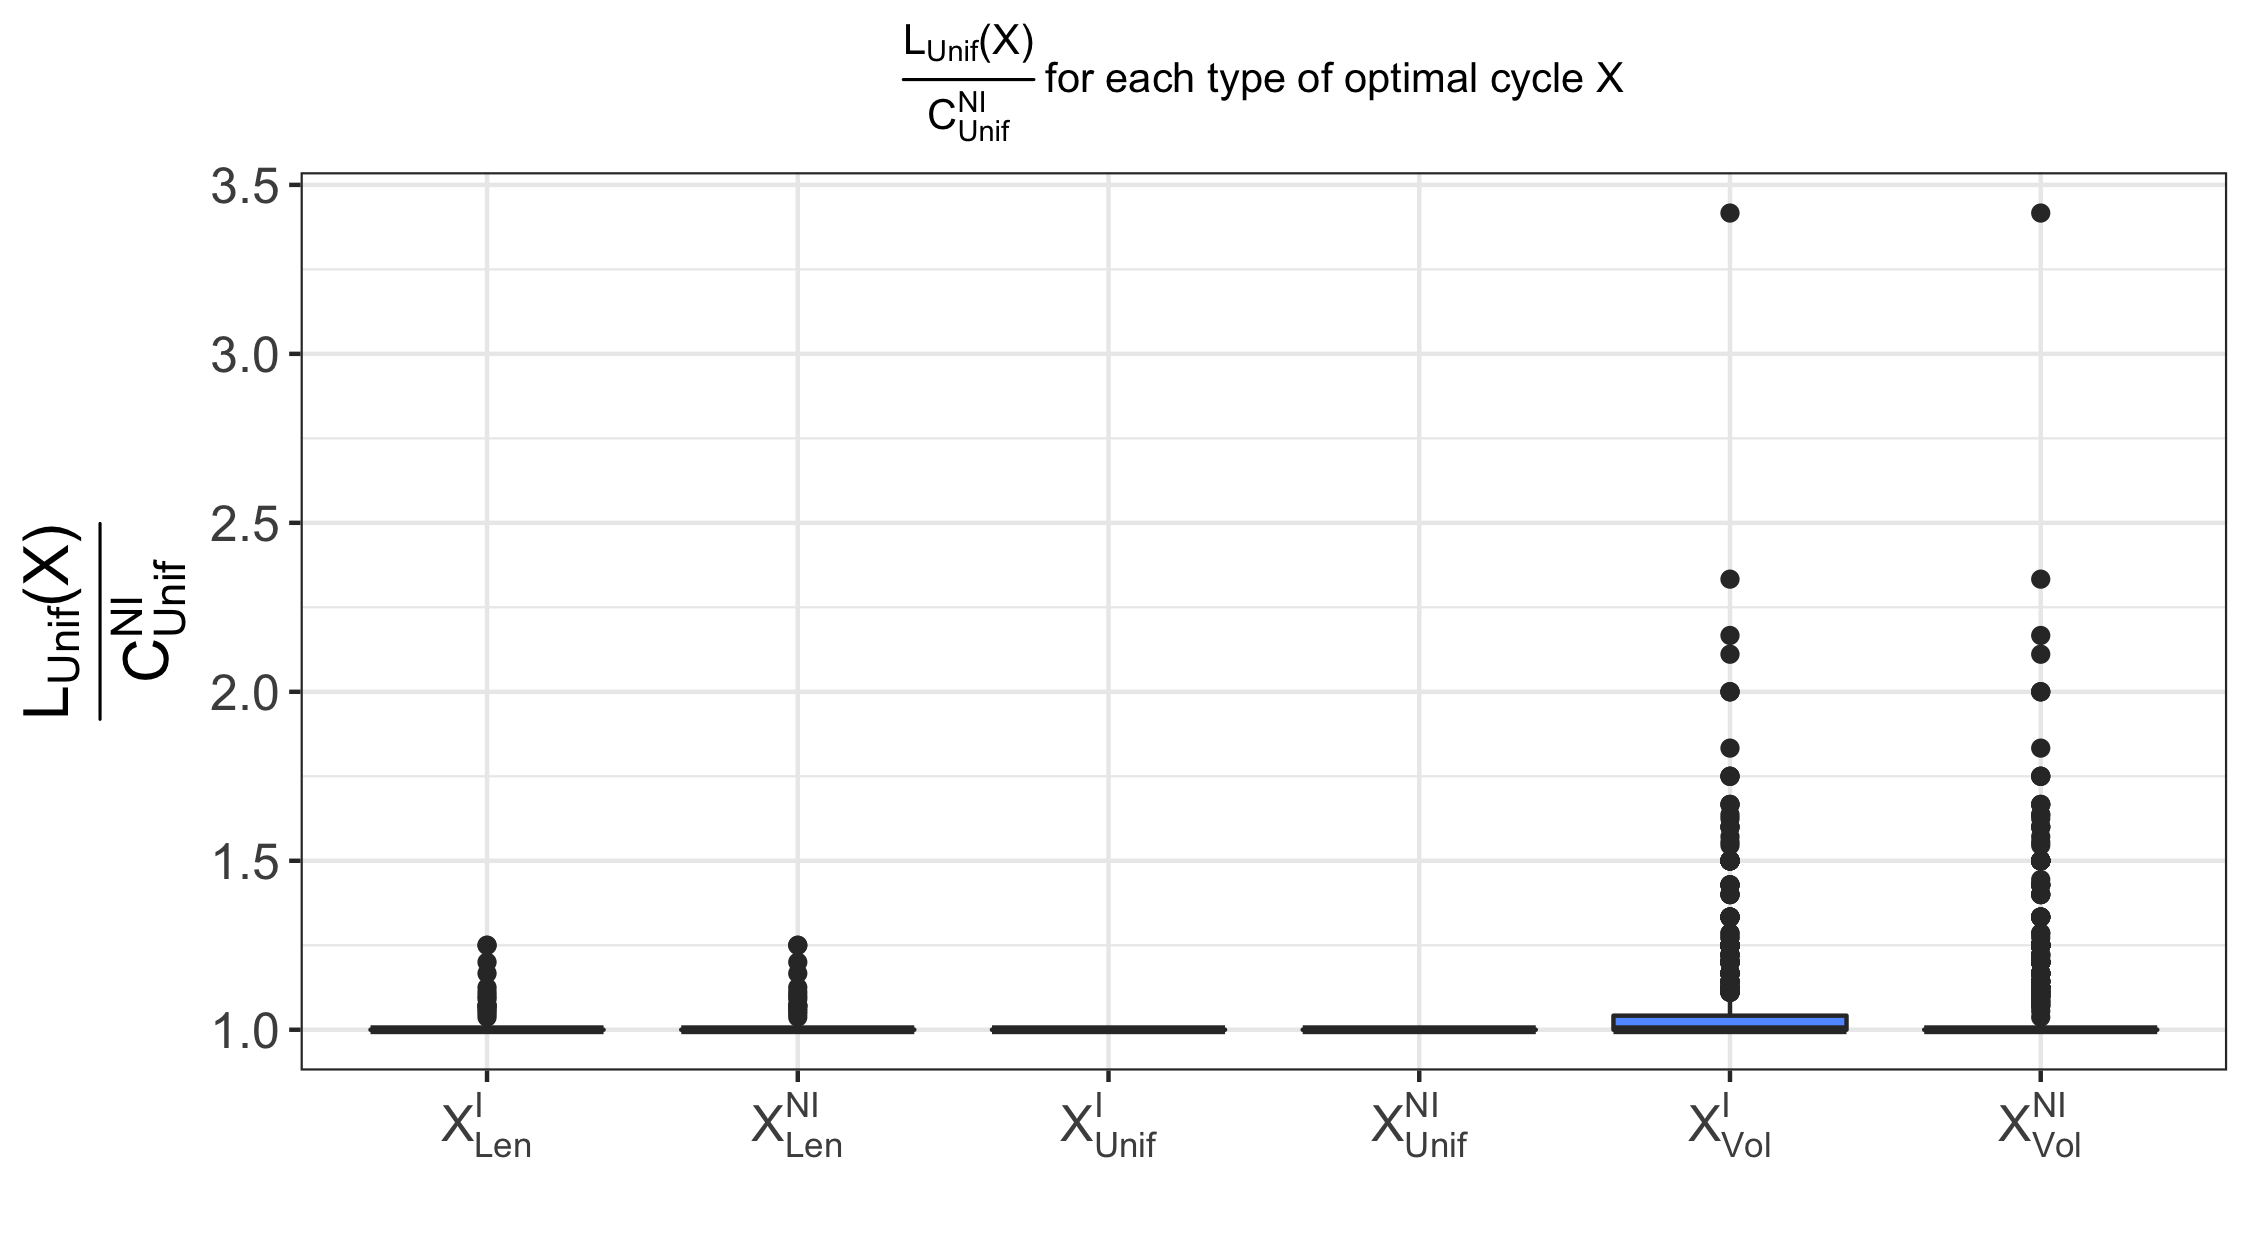
\includegraphics[width=\textwidth]{figures/edge_compare.png}
% \end{center}
% \caption{Box plots comparing the uniform-weighted loss of each type of optimal cycles against the uniform-weighted optimum cost. The $x$-axis is the type of optimal cycle and the $y$-axis is the ratio between the uniform-weighted cost of each type of optimal cycle and the actual uniform-weighted cost of the uniform-weighted minimal cycle (i.e. the number of edges in the cycle) without requiring integral solutions. We expect the middle two columns to be 1 as the optimums obtained whether requiring integral solutions or not are the same in all our experiments.}\label{fig:edgecompare}
% \end{figure}